Изначально искусственные нейронные сети строились как модель коры головного мозга человека. 
В отличие от своего биологического аналога нейронная сеть, как правило, имеет дифференцируемые функции 
активации, необходимые для эффективного обучения в ходе обратного распространения ошибки.

\textit{Определение:} \textbf{Функцией активации} в нейронной сети называется \textit{нелинейная} функция,
связывающая выходной сигнал и активацию нейрона. 

На практике широко используются функции активации в виде сигмоидов $\sigma(x)$, ReLU \cite{agarap2018deep} и 
GeLU \cite{hendrycks2016gaussian}:
\begin{equation}
  \begin{aligned}
    & \sigma(x) = \frac{1}{1+\exp(-x)} \\
    &\text{ReLU}(x) = \min(0,x)p \\
    &\text{Tanh}(x) = \frac{e^{z}-e^{-z}}{e^{z}+e^{-z}} \\
    &\text{Gelu}(x) = \sigma(x) x 
  \end{aligned}
\end{equation}

Функция активации вводится для добавления в модель нелинейности, что позволяет нейронной сети моделировать сложные 
нелинейные зависимости в данных. Некоторые из распространенных функций активации включают в себя сигмоидальную 
функцию (\( \sigma \)), гиперболический тангенс (\( \tanh \)), ReLU (Rectified Linear Unit) и их вариации.

\textit{Определение:} Перцептроном называется параметрическая математическая модель нейрона. Перцептрон
задается матрицей весов $W$, смещением $b$ и функцией активации $\sigma$:
\begin{equation}
  \mathbf{y} = \sigma(W \mathbf{x} + \vec{b})
\end{equation}

\begin{figure}[h]
  \centering
  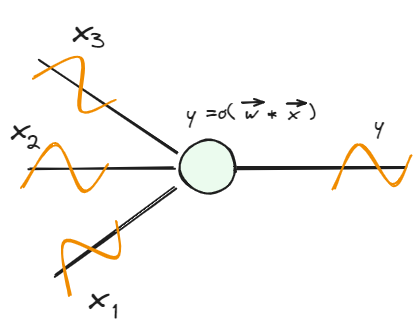
\includegraphics[width=0.5\textwidth]{assets/ml/nn/perceptron.excalidraw.png}
  \caption{Перцептрон --- базовый элемент нейронной сети}
  \label{perceptron}
\end{figure}

\textit{Определение:} \textbf{Нейронные сети} --- параметрическая аппроксимирующая данные модель, состоящая из упорядоченных слоев
обучаемых слоев перцептронов:
\begin{equation}
  f^i(W^i f^{i-1}(W^{i-1} \dots f^1(W^1(x)))),
\end{equation}
где $f^i$ --- функция активации $i$-ого слоя, $W^i$ --- веса активации $i$-ого слоя.

\begin{figure}[h]
  \centering
  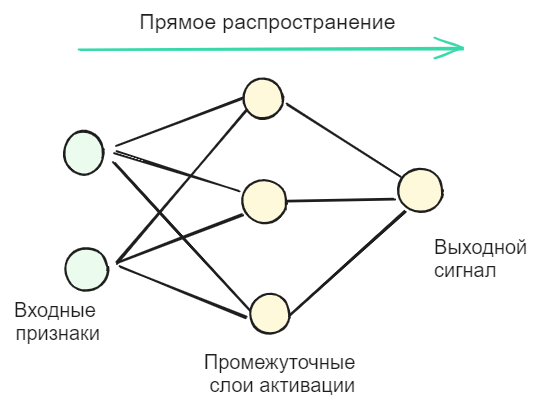
\includegraphics[width=0.5\textwidth]{assets/ml/nn/nn.excalidraw.png}
  \caption{Преобразование сигнала выполняется в промежуточных слоях активации в ходе прямого распространения сигнала}
  \label{neural_net}
\end{figure}

В случае многослойной нейронной сети, выходы нейронов одного слоя становятся входами для следующего слоя, 
образуя цепочку преобразований. Процесс распространения через нейроны последовательных слоев называется 
прямым распространением (от \textit{англ.} forward propagation).

Во время обучения модель минимизирует функцию потерь $\mathcal{L}$, которая оценивает отличие предсказанного 
результата $y_i$ от истинного значения $y_i$:
\begin{equation}
  \mathcal{L} = \frac{1}{N} \sum_{i=1}^{N} L(y_i, \hat{y}_i).
\end{equation}

Значительное число параметров в современных нейронных сетях требует
выбора численно эффективных методов оптимизации. Базовым и наиболее распространненым алгоритмом на практике является 
градиентный спуск, выполняемый с помощью методов автоматического дифференцирования \cite{paszke2017automatic}\cite{baydin2018automatic}.
Общая техника называется обратным распространением ошибки \cite{rumelhart1986learning} и основана на правиле дифференцирования
сложной функции:
\begin{equation}
  \begin{aligned}
    & \frac{\partial \mathcal{L}}{\partial w_{jk}^{(L-1)}} = \frac{1}{N} \sum_{i=1}^{N} \frac{\partial a_j^{(L)}}{\partial w_{jk}^{(L-1)}} \frac{\partial L}{\partial a_j^{L}} \\
    & \frac{\partial \mathcal{L}}{\partial \alpha^{L-1}_k} = \sum_{j=1}^{N_L} \frac{\partial{a_j^{(L)}}}{\partial{a_k}^{(L-1)}} \frac{\partial{L}}{\partial a_j^{(L)}}
  \end{aligned}
\end{equation}
где $\alpha^{L-1}_k$ --- активации $k$-перцептрона на слое $L$,  $w_{jk}^{(L-1)}$ --- вес нейрона $jk$ на слое $L$.

